\chapter{System Implementation}
\label{cha:communicationStack}
The purpose of this chapter is to show how the complexity of the system was hidden from the Application Layer through the use of methods exposed by the TRAP and Communication Layers.
\section{TRAP Layer}
\label{sec:TRAPLayer}
The TRAP Layer is the layer that implements the TRAP protocol.\\
The purpose of this layer is to allow reliable communication between nodes by reducing power failure allowing transmission only under certain conditions. Specifically, communication can only occur if the sending node and the receiving node have sufficient energy levels to send and receive the packet \cite{9733918}.\\
As the protocol is designed, this layer is based on the repeated sending at fixed intervals in time of a series of pulses that encode the node's energy level. On the other hand, the layer must receive the energy levels of neighboring nodes within the network and correctly associate them, through sending frequency recognition, with the transmitting node. For this reason, the basic implementation idea exploits timers on the MSP430 board to perform repetitive burst sending (series of pulses, varying in length depending on the energy accumulated by the node) and externals GPIO interrupts generation to handle incoming bursts.\\
To correctly associate the incoming burst with the sending node, the adopted solution is to have a timer count from the beginning of the reception and stop it at the end of the reception, then calculate the sending frequency.\\
Based on the energy level of the node and the energy level received from other nodes, the layer decides whether or not transmission can be made to and from the node.\\
\begin{figure}[H]
\centerline{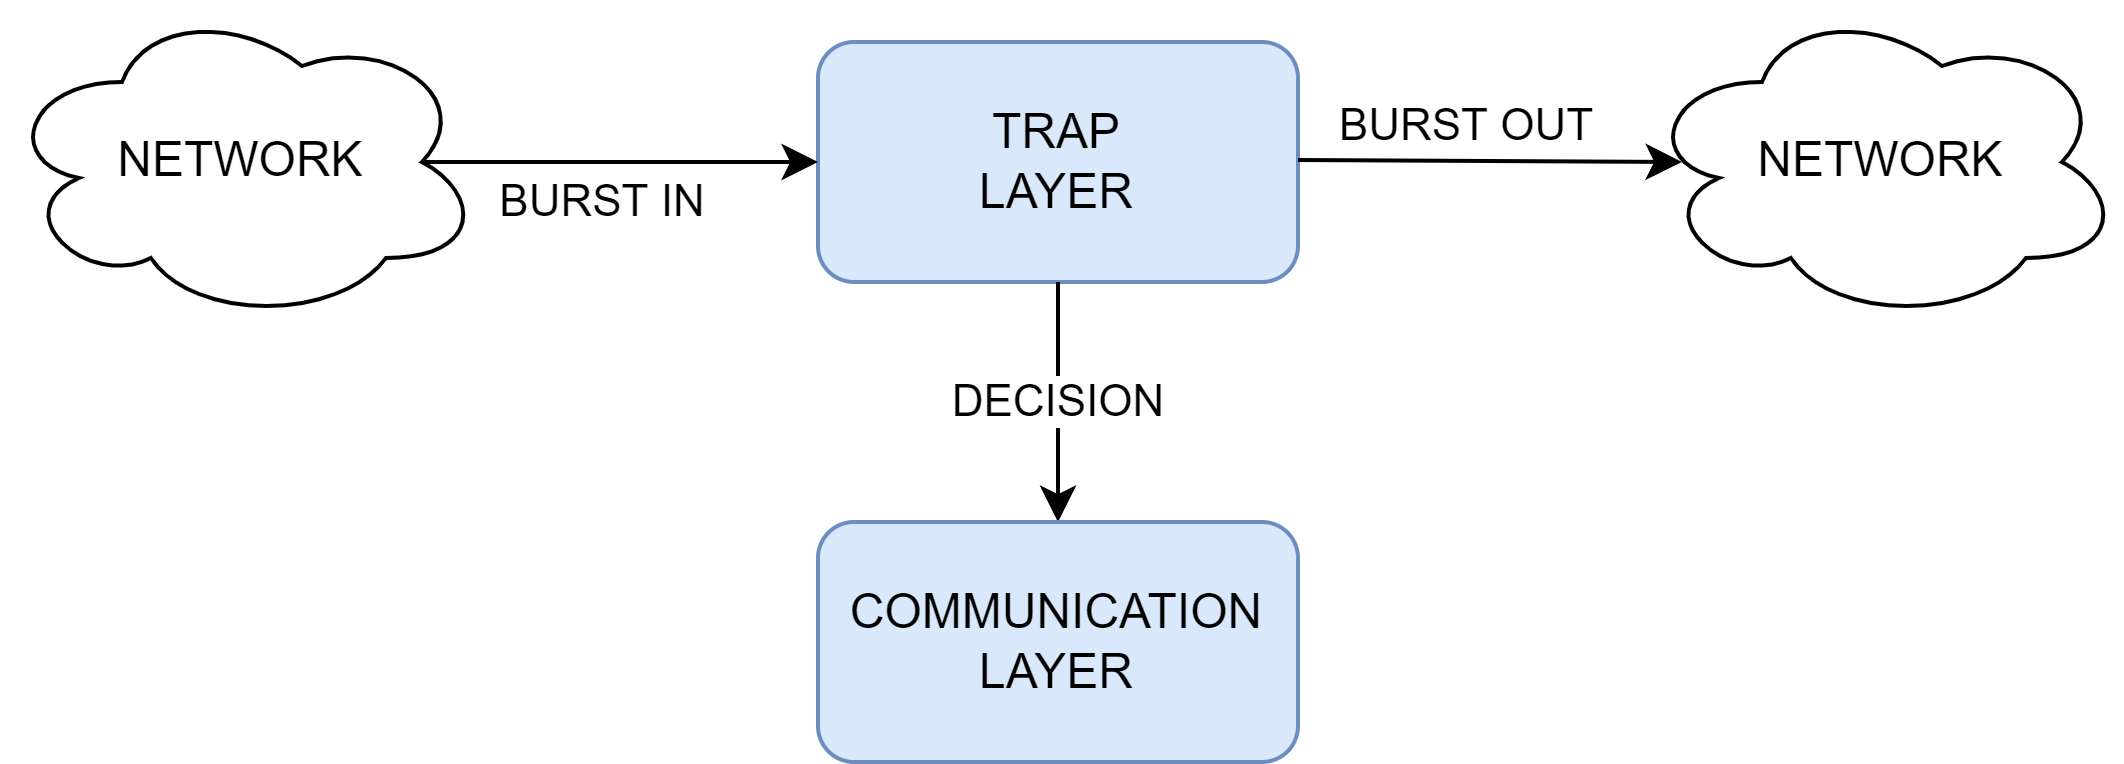
\psfig{file=Images/TRAPLayerDetails.png,width=0.7\textwidth}}
\caption{\footnotesize \centering TRAP Layer representation}
\label{fig:TRAPLayerDiagram}
\end{figure}
This Layer exposes a single function to check whether the energy level of the sending node and the receiving node is sufficient to complete the transmission. The return value of the method is 1 if sending is possible, and 0 otherwise.
\section{Communication Layer}
\label{sec:CommunicationLayer}
This section of the system contains the infrastructure needed to limit the loss of data and consequently the waste of energy following a power failure. More specifically: saving data to non-volatile memory, restoring data from non-volatile memory, sending data to the Physical Layer, sending data to the Application Layer, and checking data validity in case of expired packets.\\
Control over packet expiration is included within the sending of data to the Physical Layer and the Application Layer. For this reason, it will be discussed in those sections and not in a dedicated part.\\
Before analyzing the implementation choices in detail, it is convenient to indicate the package structure used by the layer for processing.
\subsection{Packet Structure}
\label{sec:PacketStruct}
 The package is defined as follows:
\begin{table}[H]
\begin{center}
\begin{tabular}{ |c| c| c| c| c| c| c| c|}
 NODEID & DATA0 & DATA1 & DATA2 & DATA3 & CRC0 & CRC1 & TIMESTAMP\\ 
\end{tabular}
\caption{\label{tab:Packet format}Package structure, 64bit}
\end{center}
\end{table}
The packet consists of 8 byte-sized fields. Specifically, the first field indicates the producing node, the next four the data produced, then we find two CRC fields used to detect any errors in transmission, while the last field indicates the production timestamp of the packet.\\
It is important to note that the fields are byte-sized, this allows atomic operations in memory.
\subsection{Data Saving From Application Layer (Data saving TX)}
\label{sec:CommLayer1}
The Application Layer calls the producedData() method passing as arguments four bytes of data and one byte indicating the message recipient node identifier.\\
After the data reception, the Communication Layer begins saving the data in non-volatile memory.\\ 
Data saving takes place in structures containing the message fields. 
\begin{lstlisting}%
[caption={Structure containing the package fields and two supporting fields for managing the package in memory},label=lst:struttura,frame=trbl]
typedef struct storedData
{
    unsigned char nodeNumber, data0, data1, data2, data3, CRC0, CRC1, timeStamp, saved, nodeRX;
} storedData;
\end{lstlisting}
These structures are arranged in a circular buffer (Buffer TX). 
For this purpose, it is important to keep track of the last location written to the buffer in case of power failure. 
This is needed to avoid inadvertent overwriting of data. 
To do this it is necessary to save in non-volatile memory a field that will serve as a pointer.\\
The four data passed to the function are saved directly, byte by byte, in non-volatile memory along with the producer node value (the latter value is already known to the Communication Layer and does not need to be passed by the Application Layer).\\
Next, the Communication Layer proceeds to calculate the CRC16 value of the four bytes of data passed by the Application Layer. The resulting two bytes are saved in non-volatile memory too.\\
At this point, the packet time stamp, and the recipient node identifier are added.\\
The packet will be confirmed as saved by setting a control byte to 1 and incrementing the buffer pointer.\\
Finite state machine of data saving from Application Layer is presented in Figure \ref{fig:FSMSAVETX}.\\
If no power failure is encountered during saving, the package is saved correctly and ready to be sent when requested by the application layer.\\
On the contrary, any power failure before the pointer increment would render the data unusable and would be overwritten at the next save request by the Application Layer.\\
\begin{figure}[H]
\centerline{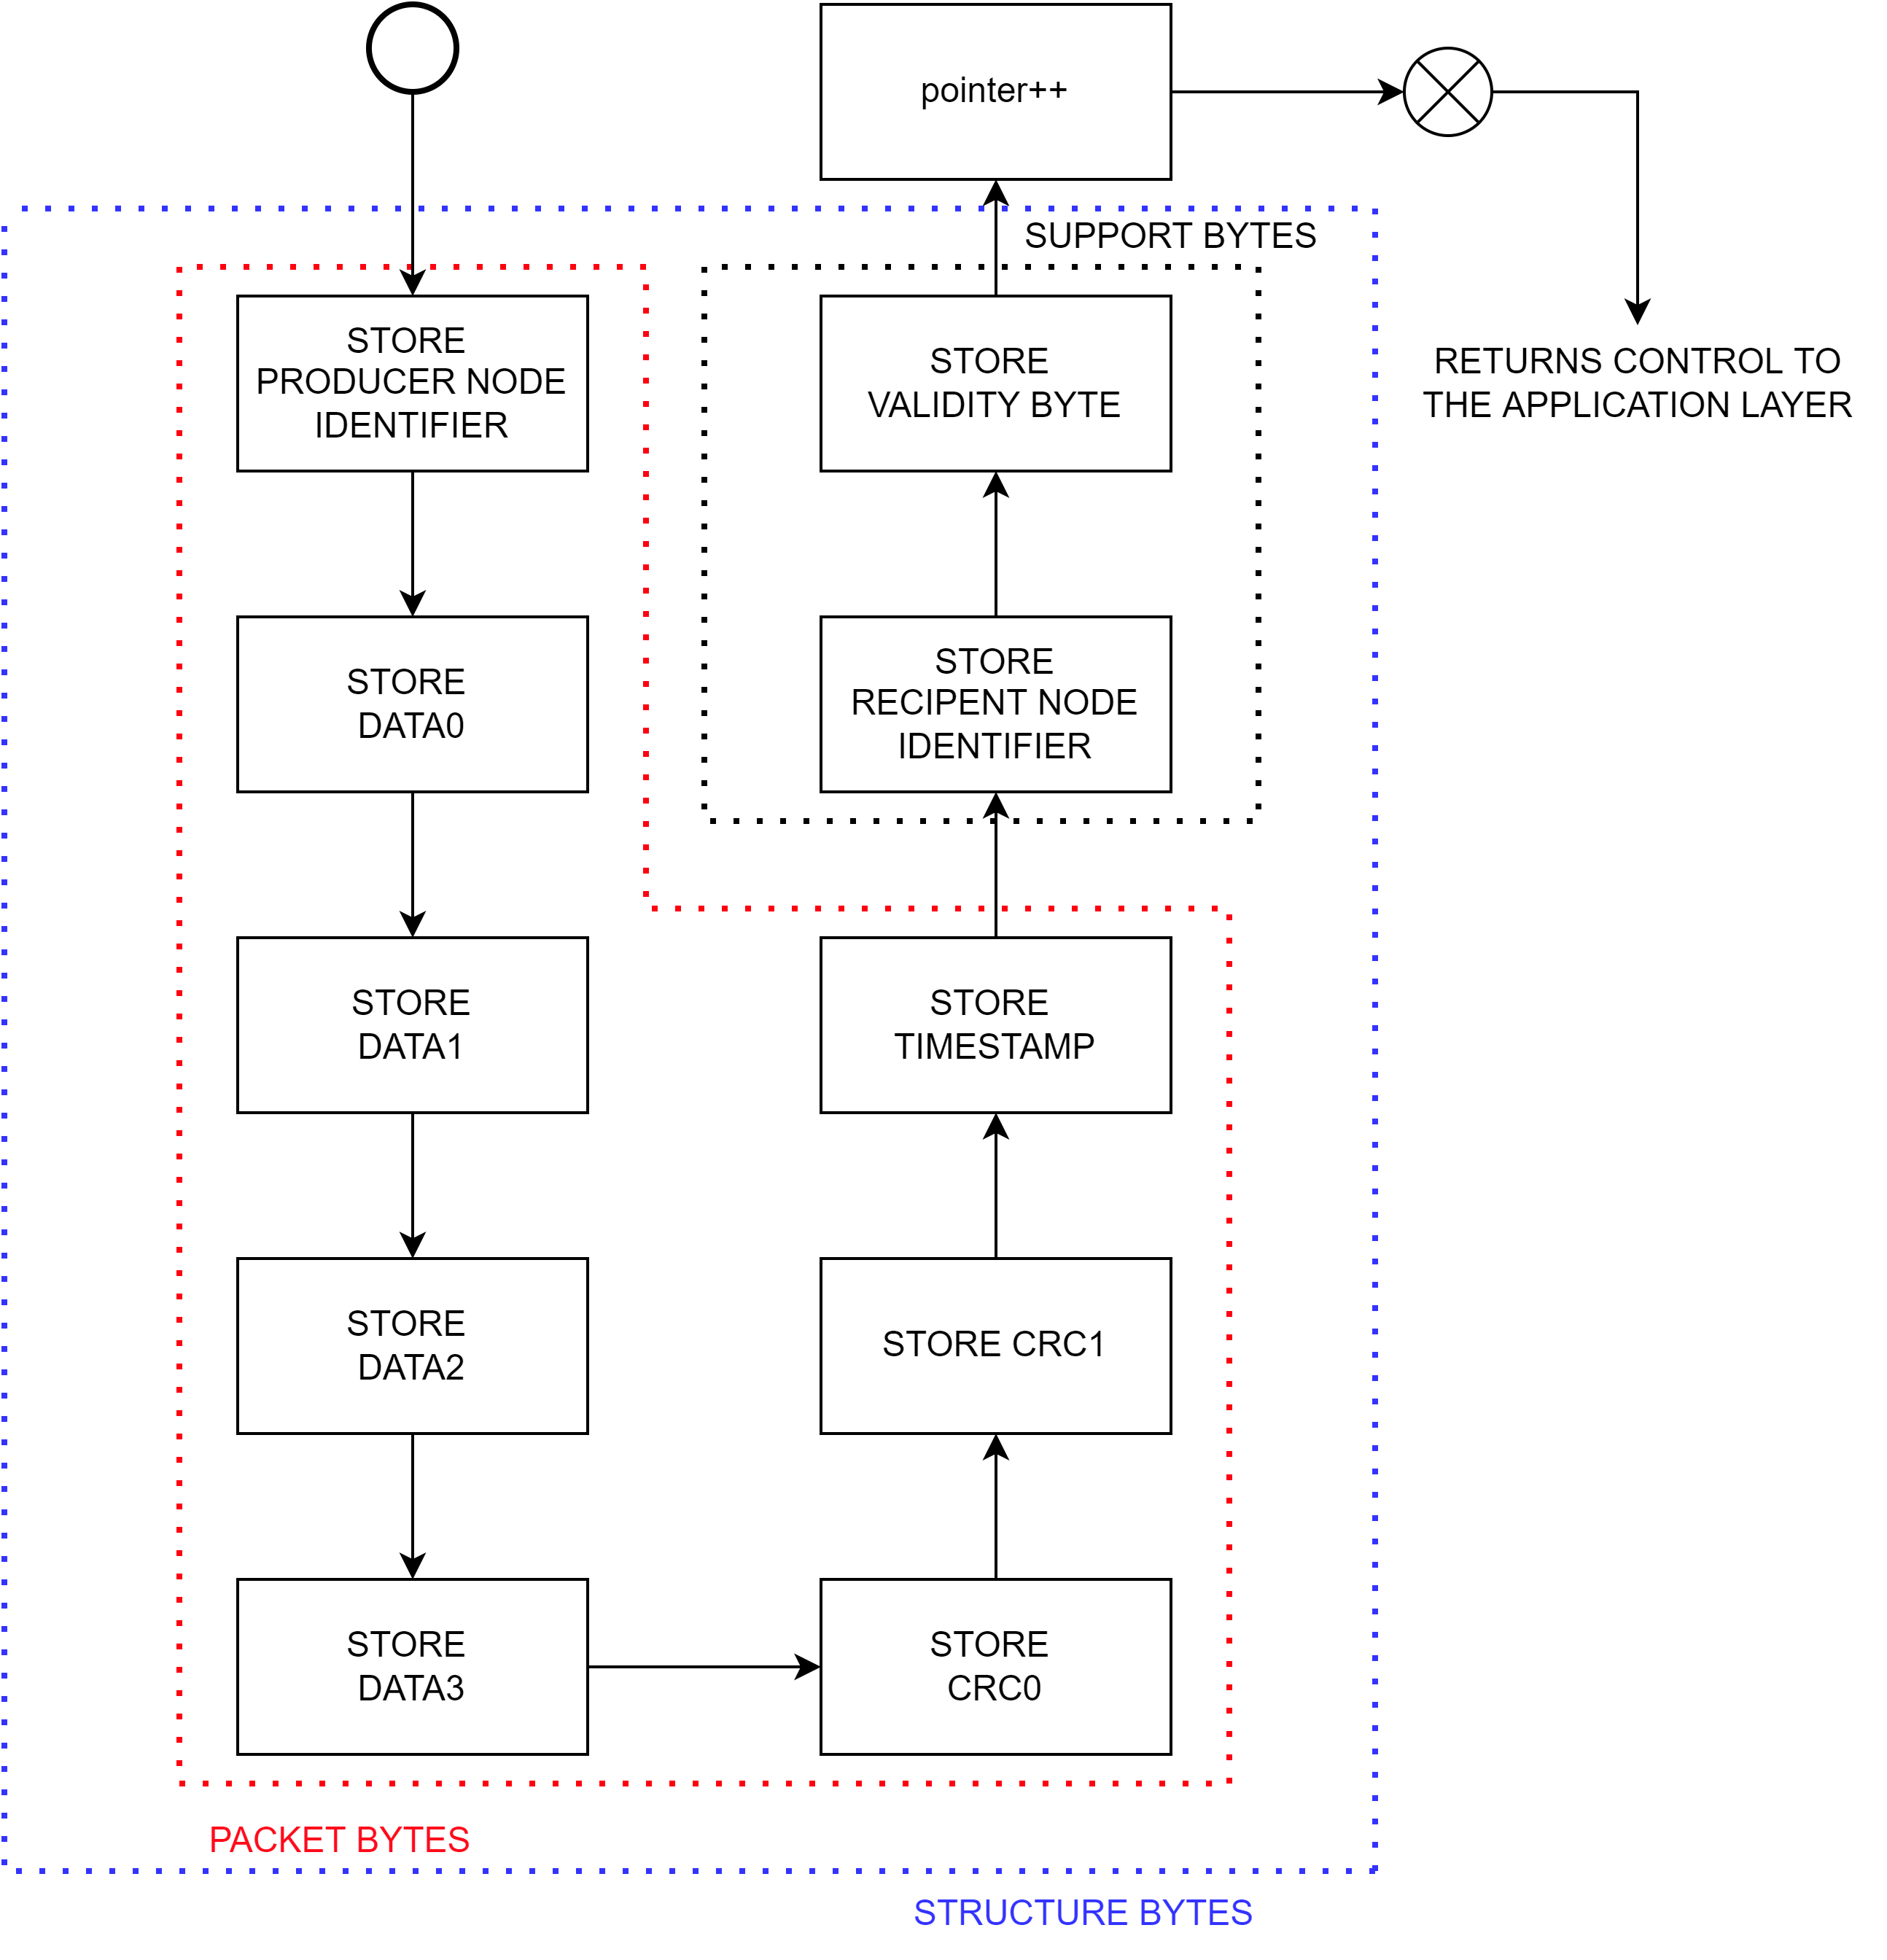
\psfig{file=Images/SaveTX-FSM.png,width=0.8\textwidth}}
\caption{\footnotesize \centering Finite state machine related to package building and saving (pointer: writePointer)}
\label{fig:FSMSAVETX}
\end{figure}
\subsection{Data Sending To Physical Layer (Data TX)}
\label{sec:CommLayer2}
To send the data produced, the Application Layer must call the dataSend() method without passing arguments.\\
When this method is invoked, the Communication Layer chooses the packet stored in non-volatile memory to send and forwards it to the Physical Layer.\\
The selection of the packet to be sent is the most relevant section of this method.
The packets to be sent are stored in a circular buffer, so you have to keep track of the packet by a pointer stored in non-volatile memory. The logic is the same as shown in the data saving. The pointer is incremented only when the operation is completed and the validity byte is reset to 0. This is important in case of power failure, if the control byte was reset before the sending was completed, the packet would be marked as sent when in fact it was not.\\
The data is considered valid only if the control byte (set during packet saving) is set to 1.\\
Choosing the packet to be sent only with the pointer, however, is not the best solution. 
In fact, before each send, the canSendTRAP() method of the TRAP layer is called to check whether it can be transmitted to the recipient node.\\
If a recipient node A shuts down and the buffer contains messages for nodes A, B and C in that order, the insufficient energy level of A blocks the messages for B and C. In order to avoid that, the node sends the next packet in the buffer (i.e. the one for B), if possible, otherwise it tries with the next again and so on.\\
The solution adopted involves a priority check on the packet indicated by the pointer. If it cannot be sent, checks are made on subsequent packets until a sendable packet is reached or the entire buffer is scrolled (Figure \ref{fig:FSMSENDTX}).
\begin{figure}[H]
\centerline{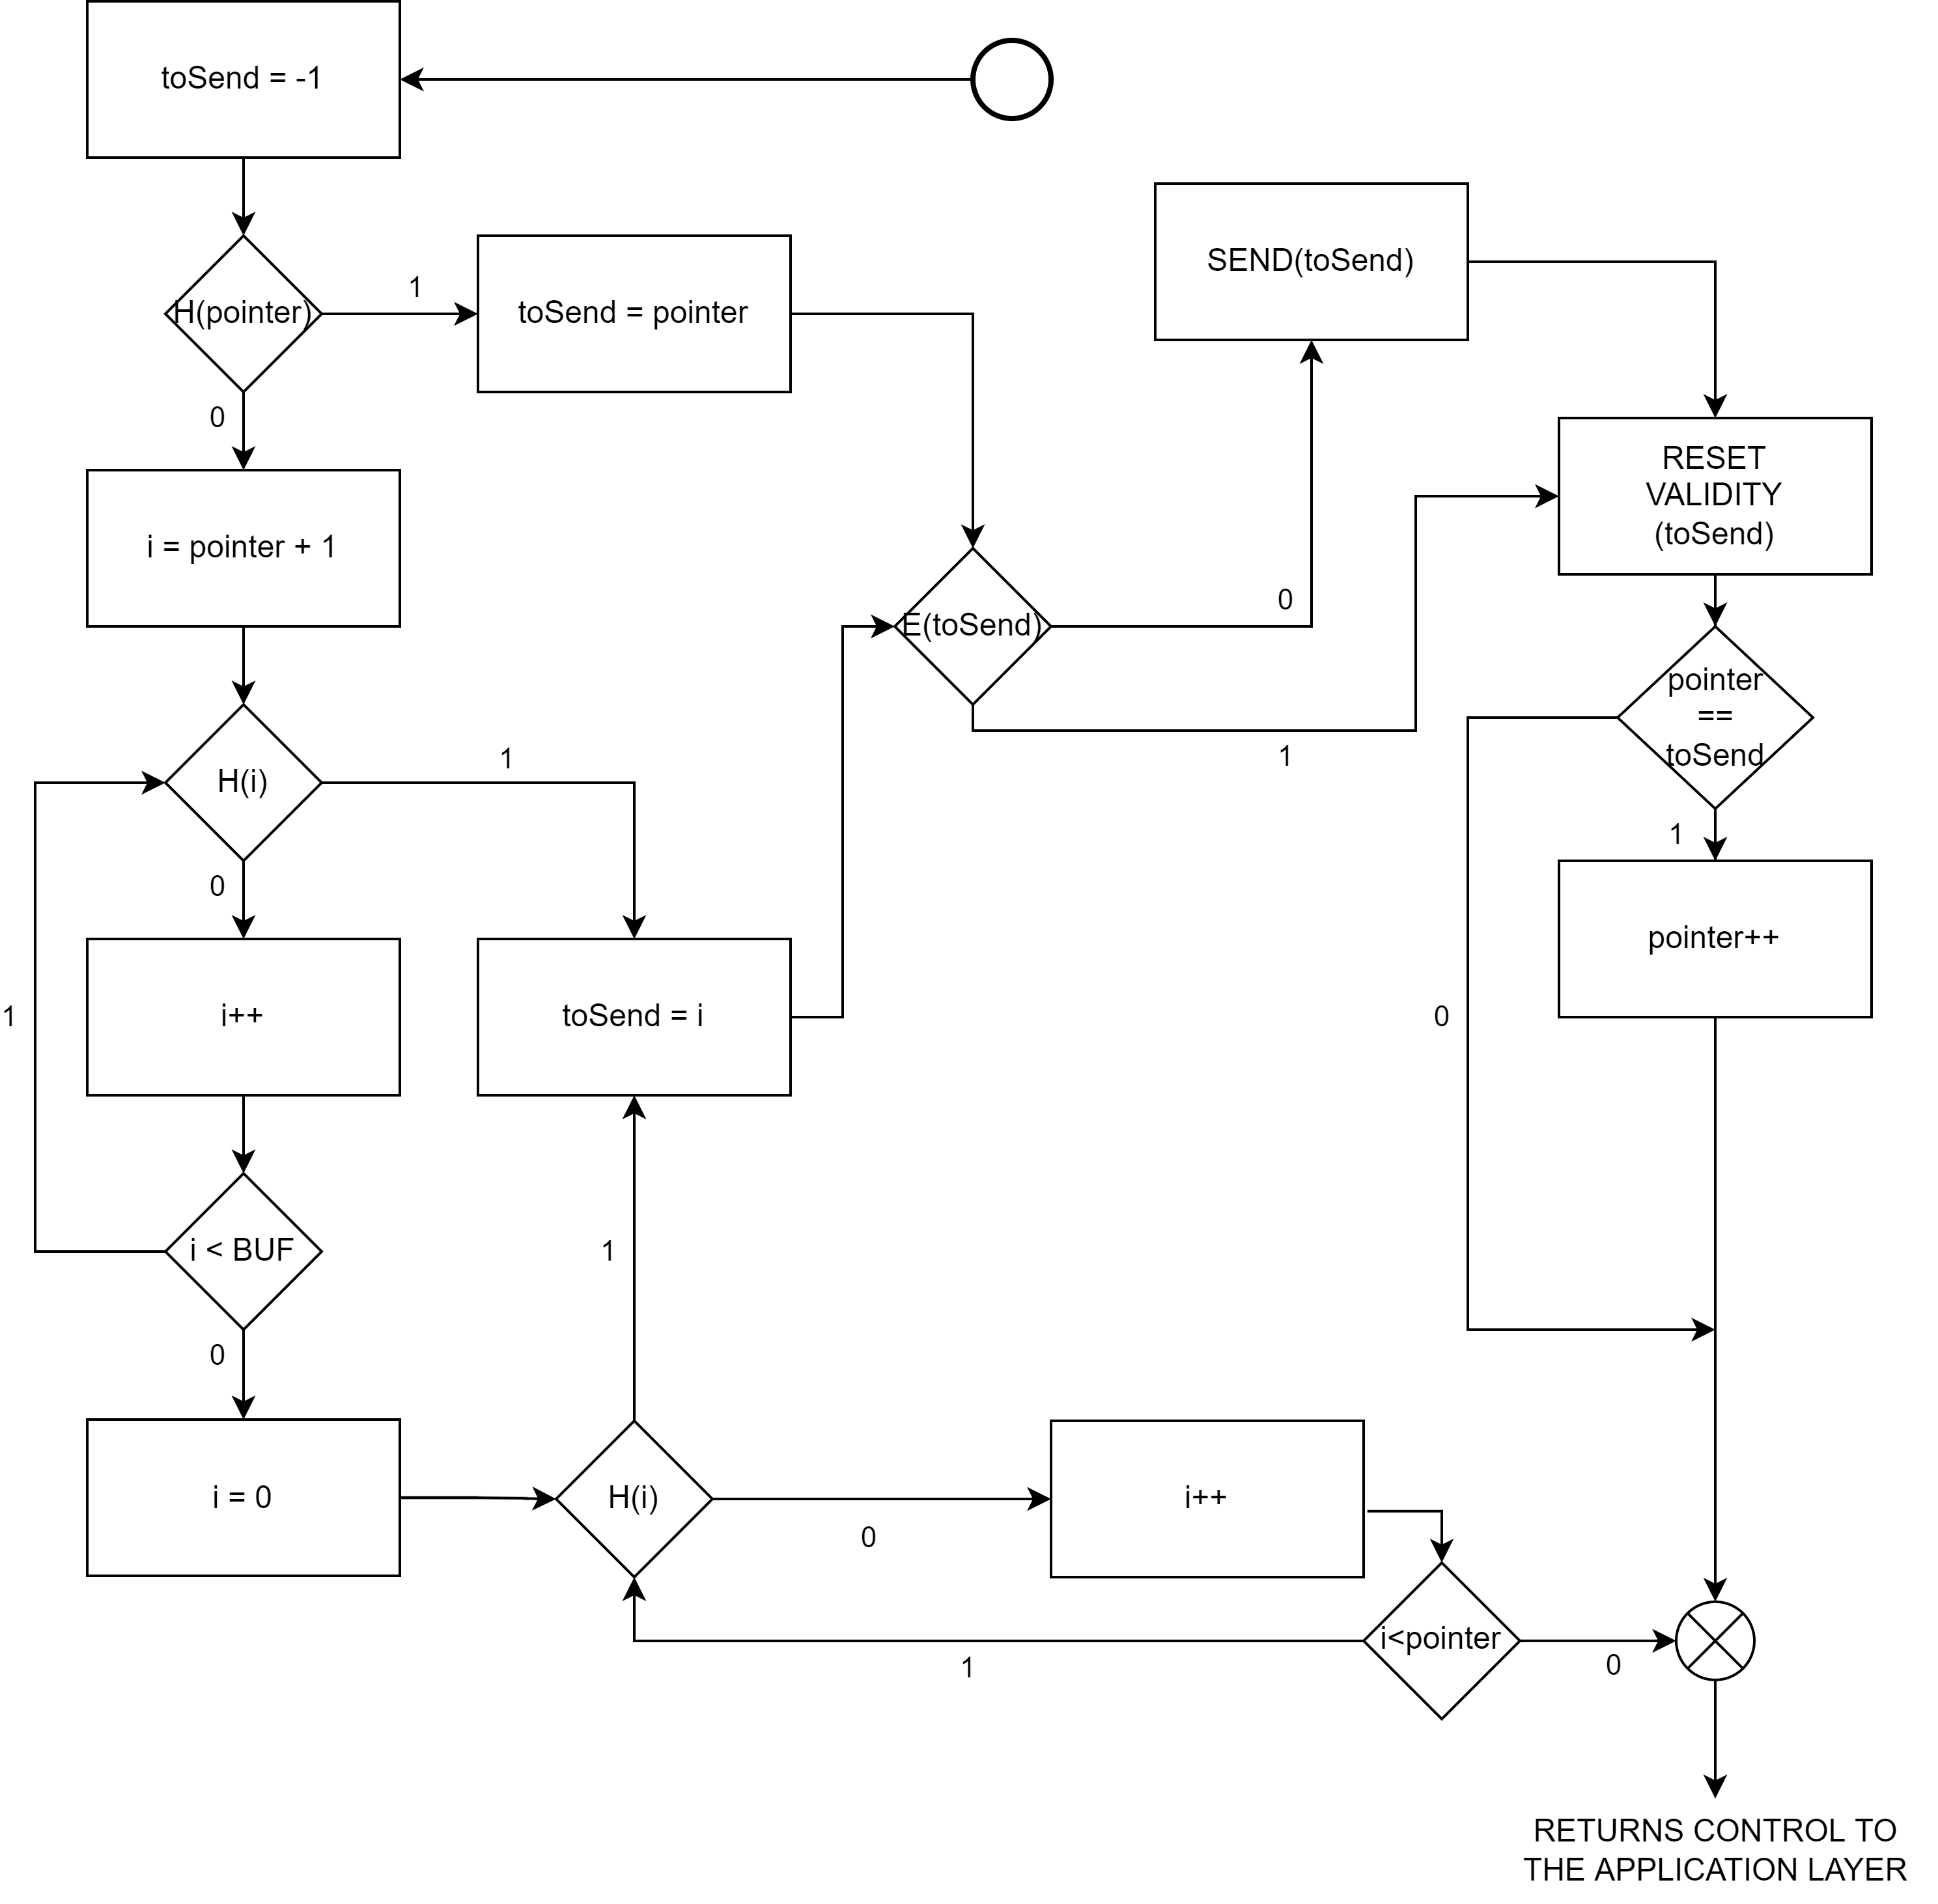
\psfig{file=Images/sendTX-FSM.png,width=0.75\textwidth}}
\caption{\footnotesize \centering Finite state machine related to package selection and sending (H(x): (checkValidity(x) \&\& canSendTRAP(x)), E(x): expiration(x), pointer: sendPointer, BUF: TX Buffer size)}
\label{fig:FSMSENDTX}
\end{figure}
\subsection{Data Saving From Physical Layer (Data saving RX)}
\label{sec:CommLayer3}
Saving data received from the Physical Layer is done in much the same way as presented for saving data from the Application Layer. Again, data saving occurs in structures containing message fields arranged within a circular buffer (Buffer RX). This requires a pointer to keep track of the last position written.\\
The Physical Layer notifies by triggering an interrupt the Communication Layer at the end of data reception.\\
The Communication Layer checks whether the received packet consists of 8 bytes. If the received packet is complete, the Communication Layer checks for errors via a CRC16 module. If no errors are detected the packet validity byte is set to 1 and the receive buffer pointer is incremented. The pointer, as explained earlier, is not incremented before packet acknowledgment because in case of power failure it could lead to marking inconsistent packets as good.
\begin{figure}[H]
\centerline{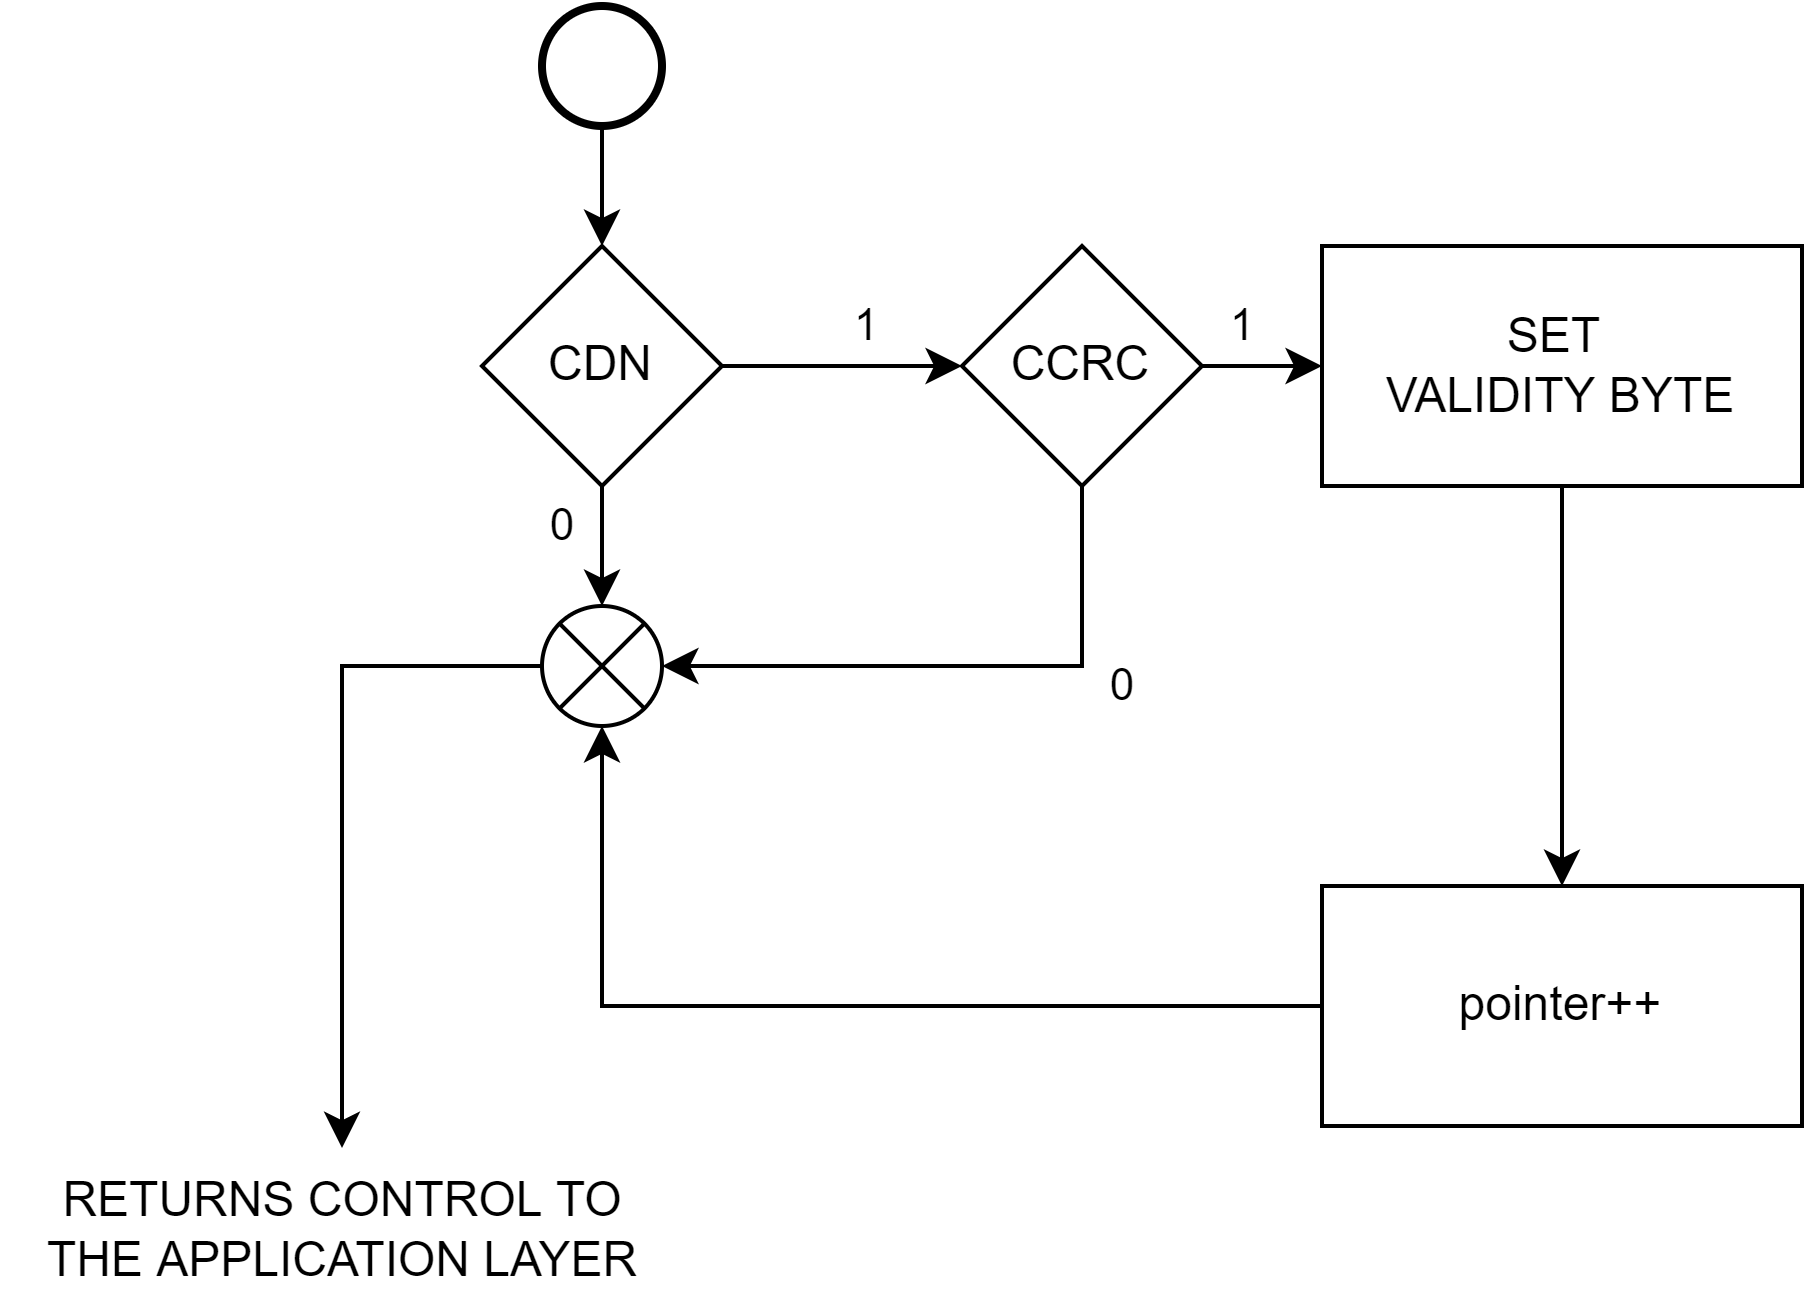
\psfig{file=Images/saveRX-FSM.png,width=0.65\textwidth}}
\caption{\footnotesize \centering Finite state machine related to Data saving RX (CDN: checkDataNumber(), CCRC: checkCRC())}
\label{fig:FSMSAVERX}
\end{figure}
\subsection{Data Sending To Application Layer (Data RX)}
\label{sec:CommLayer4}
The forwarding of packets from the Communication Layer to the Application Layer is done by the call of the getData() function.\\
The Application Layer receives a structure containing the first available packet saved in memory if present, a packet initialized to zero otherwise.\\
When the getData() function is called, the Communication Layer scrolls through all the packets saved in the RX buffer to delete the expired ones.\\
Thereafter, the packet choice is made similarly to what was seen for sending to the Physical Layer. The difference, concerning what was presented earlier, is related to the TRAP check that does not have to be performed.\\
For the location of the packet to be transmitted within the buffer, a pointer is saved in non-volatile memory. This pointer will be incremented only after the validity byte of the structure containing the data is reset.
\begin{figure}[H]
\centerline{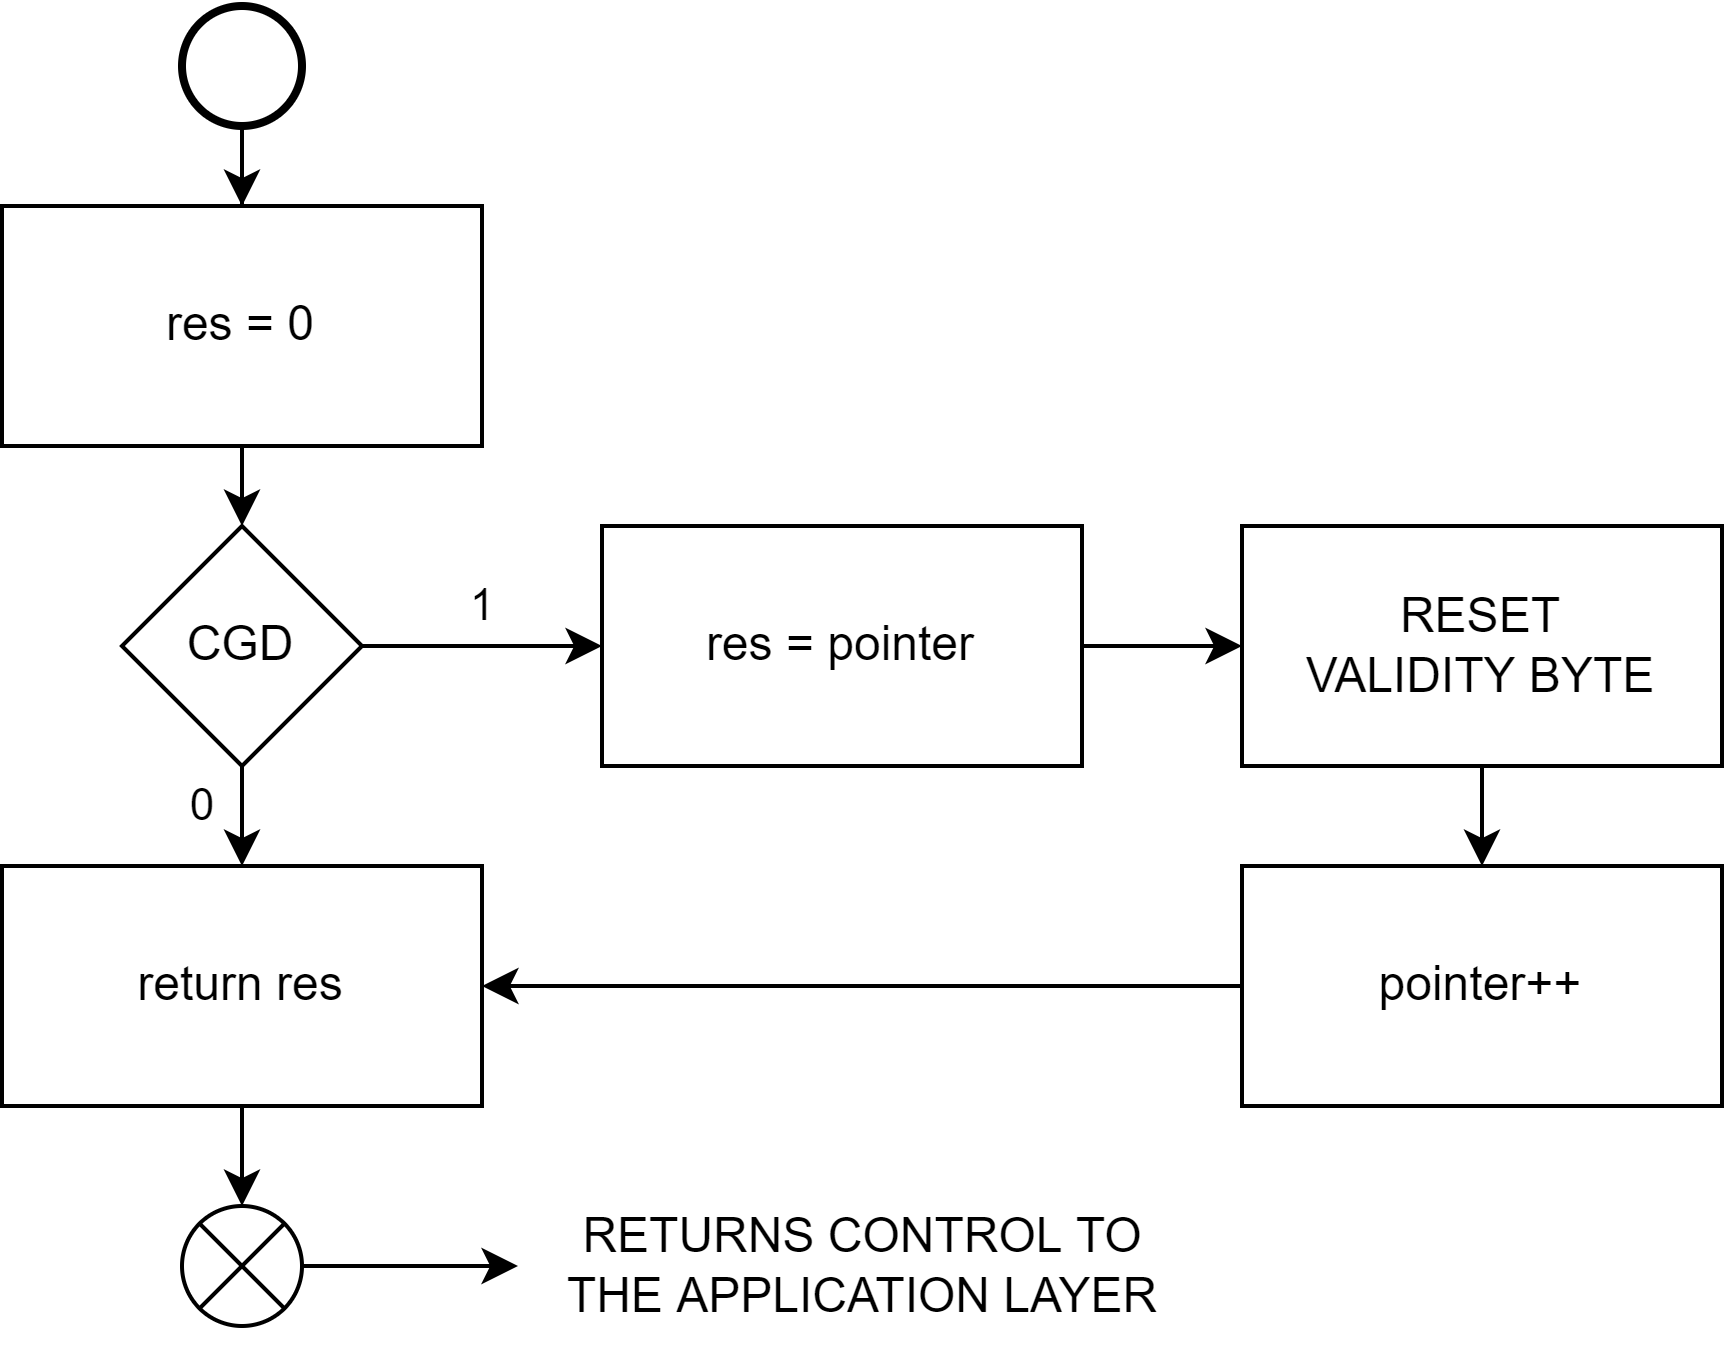
\psfig{file=Images/dataGet.png,width=0.65\textwidth}}
\caption{\footnotesize \centering Finite state machine related to getData() function (CGD: canGetData())}
\label{fig:DATAGET}
\end{figure}
\section{Power Failure Resistance}
\label{sec:PowerFailureResistance}
Since power failure resilience is the novelty of this thesis, it is worth spending a few words explaining what happens in case of power failure during normal system operation such as during sending data from the Application Layer to the Communication Layer, forwarding data from the Communication Layer to the Physical Layer for sending to the network, receiving data from the network to the Physical Layer and forwarding to Communication Layer, and during data sending from the Communication Layer to the Application Layer.\\
\subsection{From The Application Layer To The Communication Layer}
In this case, we have several possibilities:
\begin{enumerate}
\item Power failure occurs before the packet is acknowledged through the validity byte set
\item Power failure occurs immediately after the packet validity byte set but before the pointer increment that signals the location to be written to the buffer
\item Power failure occurs after the packet validity byte set and after the pointer increment that signals the location to be written to the buffer (just before the return from the function to the Application Layer)
\end{enumerate}
In the first scenario, the partially saved packet will be overwritten at the next data pass by the Application Layer. This is the worst situation because the data cannot be sent. The energy used to produce it has been wasted.\\\\
In the second scenario, the situation is slightly better than shown above. The packet will, again, be overwritten on the next pass of data by the Application Layer. However, having the validity byte set to 1 makes it possible to send it if it is not overwritten first. This operation could be useful when the Application Layer produces less data than can be sent as it would still allow the packet to be sent. The power produced to produce the data is considered lost only if the packet is overwritten.\\\\
In the third situation, the power failure is of no consequence since the packet is marked as saved correctly and thus can be sent following the Application Layer request. Similarly, the pointer to the buffer location is incremented, consequently, a new data save call by the Application Layer would not overwrite the packet since the next location in the buffer would be written.\\
\subsection{From The Communication Layer To the Physical Layer}
A power failure during data transfer from the Communication Layer to the Physical Layer is a remote possibility; in fact, this transfer is either authorized or denied by the TRAP protocol.\\
However, developing a system that relies only on the TRAP protocol and has no persistent management of packets to be sent does not seem like a good solution.\\
Therefore, we can consider and show how packets are handled in case of power failure during sending from the Communication Layer to the Physical Layer. It should be remembered that sending data from the Communication Layer to the Physical Layer occurs only when the TRAP protocol responds affirmatively to the possibility of sending the packet to a particular node. Data sent to the Physical Layer is immediately forwarded to the recipient node.\\
In this case, we have several possibilities:
\begin{enumerate}
\item Power failure occurs before the packet validity byte is reset
\item Power failure occurs after the reset of the packet validity byte
\end{enumerate}
In the first case, the packet is not marked as sent since the validity byte is not changed. The packet will be resent when possible. The power used to send part of the packet is lost.\\\\
In the second case, the validity byte is reset, and then a power failure occurs. The way the stack is implemented, if the validity byte is set to zero, the packet can no longer be sent and will be overwritten in subsequent saves by the Application Layer. However, resetting the byte to zero implies sending the data completely. In this situation, the pointer relative to the location in the buffer of the packet to be sent is not incremented; again, this is not a problem because the Communication Layer performs checks on the validity of the packet before forwarding it to the Physical Layer.
\subsection{From The Network To The Physical Layer}
A possible power failure during the reception of data from the Physical Layer to the Communication Layer is a situation that would be unlikely to occur; in fact, even this transmission takes place under the control of the TRAP protocol.\\
If this happens, however, the system is designed to discard the packet if it has not been marked confirmed with the validity byte set.
Specifically, the Physical Layer starts a timer upon receipt of the first piece of data. This timer is restarted with each new reception.\\
At the moment when the timer generates an interrupt, and thus no data has been received for a given time interval, the Communication Layer is called to perform a check on the amount of data that has arrived. This check is used to verify that all 64 bits of the packet have been received.\\
If a power failure occurs before the packet validity byte is set by the Communication Layer, the data is discarded and is not sent, when requested, to the Application Layer. In this case, the energy expended in receiving and transmitting the packet is wasted.
\subsection{From The Communication Layer To The Application Layer}
To receive the packet from the Communication Layer, the Application Layer must call a function that returns a packet saved in the RX buffer of the Communication Layer.\\ 
If the power failure occurs after the Communication Layer resets the packet validity byte, the packet is lost. This happens in the case where the power failure occurs during the return from the function to the Application Layer.\\
In the case, on the other hand, where the power failure occurs before the validity byte reset, the packet can be requested again at the Communication Layer since it will still be valid.
\newpage